

\noindent 
\textbf{\stepcounter{zadatak}
\thecjelina.\thezadatak.}
Tri osobe žele vući kola mase $1,2$ tona prema istoku konstantnom brzinom. Osoba $A$ vuče
silom $F_A$ iznosa $500\ N$ u pod kutom $45^\circ$ (smjer jugoistok), osoba $B$ vuče u smjeru istoka, a osoba $C$ pod kutom $30^\circ$ (smjer sjeveroistok). Koliki je iznos sila kojima vuku osobe $B$ i $C$? Koeficijent trenja između podloge i kola je $\mu_k=0,15$.
\begin{figure}[ht]%{r}{0.7\textwidth} % Inline image example
  \begin{center}
    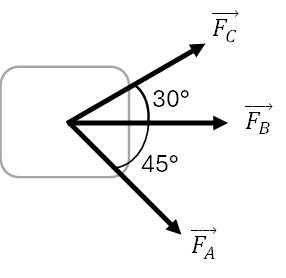
\includegraphics[scale=0.60]{../03_Dinamika_materijalne_tocke/Zadatak_D260.png}
  \end{center}
  %\caption{Fish}
\end{figure}
